\chapter{三维空间刚体运动}

\section{旋转矩阵} 

\subsection{点和向量,坐标系}

    如何表示一个点在三维空间,假设一个线性空间的基为:$(e_1, e_2, e_3)$,那么:

$$
a = 
\begin{bmatrix}
e_1, & e_2, & e_3
\end{bmatrix}
\begin{bmatrix}
a_1 \\
a_2 \\
a_3 
\end{bmatrix} = a_1e_1 + a_2e_2 + a_3e_3
$$

    对于向量的内积:

$$
    a \cdot b = a^Tb = \sum_{i = 1}^3{a_ib_i} = |a||b|cos<a, b>
$$

    对于向量的外积:

$$
a \times b = 
\begin{bmatrix}
i & j & k \\
a_1 & a_2 & a_3 \\
b_1 & b_2 & b_3 
\end{bmatrix} = 
\begin{bmatrix}
a_2b_3 - a_3b_2 \\
a_3b_1 - a_1b_3 \\
a_1b_2 - a_2b_1
\end{bmatrix} = 
\begin{bmatrix}
0 & -a_3 & a_2 \\
a_3 & 0 & -a_1 \\
-a_2 & a_1 & 0
\end{bmatrix}b \triangleq a^\land b
$$

    外积的方向垂直于这两个方向,大小为$|a||b|sin<a, b>$。对于外积,此处引入了${}^\land$符号,把$a$携程一个矩阵。事实上是一个反对称矩阵($Skew-symmetric$),可以将${}^\land$记成一个反对称符号。

    外积只对三维向量存在定义,可以用外积表示向量的旋转

\subsection{坐标系间的欧式变换}

\begin{quote}
    \centering
    描述两个坐标系之间的旋转关系,加上平移统称为坐标系之间的变换关系
\end{quote}

\begin{figure}[!htbp]
    \centering
    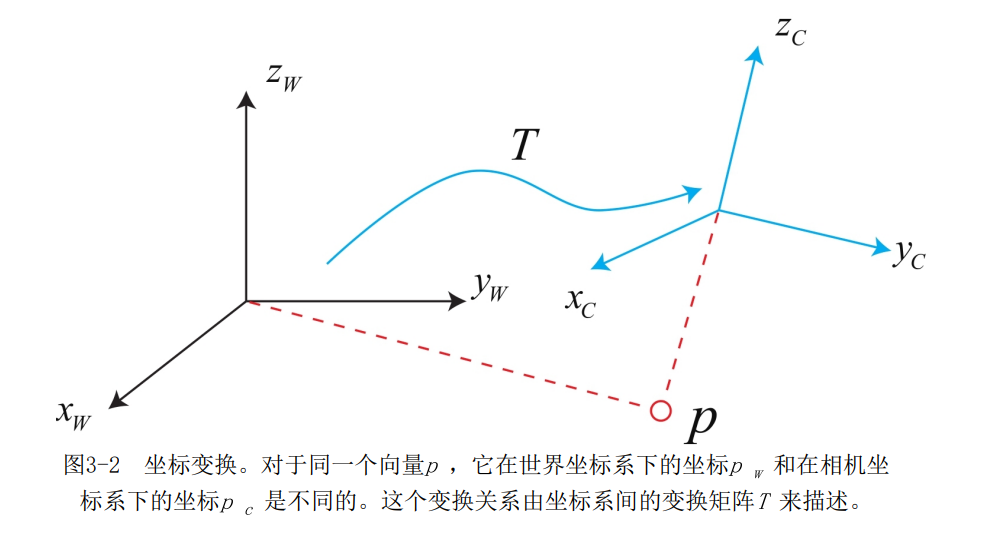
\includegraphics[width=0.3\textwidth]{image/chapter02/坐标系的旋转.png}
    \caption{坐标系的旋转}
\end{figure}

    \emph{相机运动是一个刚体运动,保证了同一个向量再各个坐标系下的长度和角度不会发生变化},这被称为欧式变换。

    一个欧式变换由\emph{一个旋转和一个平移两部分组成}。首先考虑旋转,我们设某个单位正交基$(e_1, e_2, e_3)$经过一次旋转变为$(e_1^{'}, e_2^{'}, e_3^{'})$,那么对于同一个向量$a$(\emph{该向量并没有随着坐标系的旋转而发生运动}),它再这两个坐标系下的坐标分别为:$\begin{bmatrix}a_1, & a_2, & a_3\end{bmatrix}^T$和$\begin{bmatrix}a_1^{'}, & a_2^{'}, & a_3^{'}\end{bmatrix}^T$,那么就有:

$$
\begin{bmatrix}
    e_1, & e_2, & e_3
\end{bmatrix}
\begin{bmatrix}
    a_1 \\ a_2 \\ a_3
\end{bmatrix} = 
\begin{bmatrix}
    e_1^{'}, & e_2^{'}, & e_3^{'}
\end{bmatrix}
\begin{bmatrix}
    a_1^{'} \\ a_2^{'} \\ a_3^{'}
\end{bmatrix}
$$

    此时将上述等式的左右两边同时乘上$\begin{bmatrix}e_1^{T} \\ e_2^{T} \\ e_3^{T}\end{bmatrix}$:

$$
\begin{bmatrix}
    a_1 \\ a_2 \\ a_3
\end{bmatrix} = 
\begin{bmatrix}
    e_1^Te_1^{'}, & e_1^Te_2^{'}, & e_1^Te_3^{'} \\
    e_2^Te_1^{'}, & e_2^Te_2^{'}, & e_2^Te_3^{'} \\
    e_3^Te_1^{'}, & e_3^Te_2^{'}, & e_3^Te_3^{'} 
\end{bmatrix}
\begin{bmatrix}
    a_1^{'} \\ a_2^{'} \\ a_3^{'}
\end{bmatrix} \triangleq Ra^{'}
$$

    我们把中间的矩阵拿出来,定义成一个矩阵$R$。\emph{这个矩阵由两组基之间的内积组成,刻画了旋转前后同一个向量的坐标变换关系}。只要旋转是一样的,这个矩阵也是一样的。\emph{可以说,矩阵$R$描述了旋转本身,因此又称为旋转矩阵}

    旋转矩阵本身有一些特别的性质,比如它是一个行列式为1的正交矩阵,反之,行列式为1的正交矩阵也是一个旋转矩阵。因此,可以定义:

$$
	SO(n) = \{R \in \mathbb{R}^{n \times n} | RR^T = I, det(R) = 1 \}
$$

    $SO(n)$是特殊正交群($Special Orthogonal Group$)的意思(下一讲)。\emph{旋转矩阵可以描述相机的旋转}

